\documentclass[a4paper,12pt]{article} % This defines the style of your paper

\usepackage[top = 2.5cm, bottom = 2.5cm, left = 2.5cm, right = 2.5cm]{geometry} 
\usepackage[utf8]{inputenc} %utf8 % lettere accentate da tastiera
\usepackage[english]{babel} % lingua del documento
\usepackage[T1]{fontenc} % codifica dei font

\usepackage{multirow} % Multirow is for tables with multiple rows within one 
%cell.
\usepackage{booktabs} % For even nicer tables.

\usepackage{graphicx} 

\usepackage{setspace}
\setlength{\parindent}{0in}

\usepackage{float}

\usepackage{fancyhdr}

\usepackage{caption}
\usepackage{amssymb}
\usepackage{amsmath}
\usepackage{mathtools}
\usepackage{color}

\usepackage[hidelinks]{hyperref}
\usepackage{csquotes}
\usepackage{subfigure}

\usepackage{ifxetex,ifluatex}
\usepackage{etoolbox}
\usepackage[svgnames]{xcolor}

\usepackage{tikz}

\usepackage{framed}

\newcommand*\quotefont{\fontfamily{LinuxLibertineT-LF}} % selects Libertine as 
%the quote font


\newcommand*\quotesize{40} % if quote size changes, need a way to make shifts 
%relative
% Make commands for the quotes
\newcommand*{\openquote}
{\tikz[remember picture,overlay,xshift=-4ex,yshift=-1ex]
	\node (OQ) 
	{\quotefont\fontsize{\quotesize}{\quotesize}\selectfont``};\kern0pt}

\newcommand*{\closequote}[1]
{\tikz[remember picture,overlay,xshift=4ex,yshift=-1ex]
	\node (CQ) {\quotefont\fontsize{\quotesize}{\quotesize}\selectfont''};}

% select a colour for the shading
\colorlet{shadecolor}{WhiteSmoke}

\newcommand*\shadedauthorformat{\emph} % define format for the author argument

% Now a command to allow left, right and centre alignment of the author
\newcommand*\authoralign[1]{%
	\if#1l
	\def\authorfill{}\def\quotefill{\hfill}
	\else
	\if#1r
	\def\authorfill{\hfill}\def\quotefill{}
	\else
	\if#1c
	\gdef\authorfill{\hfill}\def\quotefill{\hfill}
	\else\typeout{Invalid option}
	\fi
	\fi
	\fi}
% wrap everything in its own environment which takes one argument (author) and 
%one optional argument
% specifying the alignment [l, r or c]
%
\newenvironment{shadequote}[2][l]%
{\authoralign{#1}
	\ifblank{#2}
	{\def\shadequoteauthor{}\def\yshift{-2ex}\def\quotefill{\hfill}}
	{\def\shadequoteauthor{\par\authorfill\shadedauthorformat{#2}}\def\yshift{2ex}}
	\begin{snugshade}\begin{quote}\openquote}
		{\shadequoteauthor\quotefill\closequote{\yshift}\end{quote}\end{snugshade}}

\newcommand{\footref}[1]{%
	$^{\ref{#1}}$%
}

\pagestyle{fancy}

\setlength\parindent{24pt}

\fancyhf{}

\lhead{\footnotesize Artificial Intelligence: Assignment 1}

\rhead{\footnotesize Giorgia Adorni}

\cfoot{\footnotesize \thepage} 


\usepackage{xcolor}
\usepackage{listings,lstautogobble}
\definecolor{gray}{gray}{0.5}
\colorlet{commentcolour}{green!50!black}
\colorlet{stringcolour}{red!60!black}
\colorlet{keywordcolour}{blue}
\colorlet{exceptioncolour}{yellow!50!red}
\colorlet{commandcolour}{magenta!90!black}
\colorlet{numpycolour}{blue!60!green}
\colorlet{literatecolour}{magenta!90!black}
\colorlet{promptcolour}{green!50!black}
\colorlet{specmethodcolour}{violet}

\newcommand*{\literatecolour}{\textcolor{literatecolour}}

\newcommand*{\pythonprompt}{\textcolor{promptcolour}{{>}{>}{>}}}

\lstdefinestyle{python}{
	language=python,
	showtabs=true,
	tab=,
	tabsize=4,
	basicstyle=\ttfamily\footnotesize,
	stringstyle=\color{stringcolour},
	showstringspaces=false,
	keywordstyle=\color{keywordcolour}\bfseries,
	emph={as,and,break,class,continue,def,yield,del,elif ,else,%
		except,exec,finally,for,from,global,if,in,%
		lambda,not,or,pass,print,raise,return,try,while,assert,with},
	emphstyle=\color{blue}\bfseries,
	emph={[2]True, False, None},
	emphstyle=[3]\color{commandcolour},
	morecomment=[s]{"""}{"""},
	commentstyle=\color{commentcolour}\slshape,
	emph={array, matmul, ones, transpose, float32},
	emphstyle=[4]\color{numpycolour},
	emph={[5]assert,yield},
	emphstyle=[5]\color{keywordcolour}\bfseries,
	emph={[6]range},
	emphstyle={[6]\color{keywordcolour}\bfseries},
	literate=*%
	{:}{{\literatecolour:}}{1}%
	{=}{{\literatecolour=}}{1}%
	{-}{{\literatecolour-}}{1}%
	{+}{{\literatecolour+}}{1}%
	{*}{{\literatecolour*}}{1}%
	{**}{{\literatecolour{**}}}2%
	{/}{{\literatecolour/}}{1}%
	{//}{{\literatecolour{//}}}2%
	{!}{{\literatecolour!}}{1}%
	{<}{{\literatecolour<}}{1}%
	{>}{{\literatecolour>}}{1}%
	{>>>}{\pythonprompt}{3},
	frame=trbl,
	rulecolor=\color{black!40},
	backgroundcolor=\color{gray!5},
	breakindent=.5\textwidth,
	frame=single,
	breaklines=true,
	basicstyle=\ttfamily\footnotesize,%
	keywordstyle=\color{keywordcolour},%
	emphstyle={[7]\color{keywordcolour}},%
	emphstyle=\color{exceptioncolour},%
	literate=*%
	{:}{{\literatecolour:}}{2}%
	{=}{{\literatecolour=}}{2}%
	{-}{{\literatecolour-}}{2}%
	{+}{{\literatecolour+}}{2}%
	{*}{{\literatecolour*}}2%
	{**}{{\literatecolour{**}}}3%
	{/}{{\literatecolour/}}{2}%
	{//}{{\literatecolour{//}}}{2}%
	{!}{{\literatecolour!}}{2}%
	{<}{{\literatecolour<}}{2}%
	{<=}{{\literatecolour{<=}}}3%
	{>}{{\literatecolour>}}{2}%
	{>=}{{\literatecolour{>=}}}3%
	{==}{{\literatecolour{==}}}3%
	{!=}{{\literatecolour{!=}}}3%
	{+=}{{\literatecolour{+=}}}3%
	{-=}{{\literatecolour{-=}}}3%
	{*=}{{\literatecolour{*=}}}3%
	{/=}{{\literatecolour{/=}}}3%
}

\lstnewenvironment{python}
{\lstset{style=python}}
{}


\begin{document}
	\thispagestyle{empty}  
	\noindent{
		\begin{tabular}{p{15cm}} 
			{\large \bf Artificial Intelligence} \\
			Università della Svizzera Italiana \\ Faculty of Informatics \\ 
			\today  \\
			\hline
			\\
		\end{tabular} 
		
		\vspace*{0.3cm} 
		
		\begin{center}
			{\Large \bf Assignment 1: \\Genetic Algorithm \& Alpha-Beta Pruning}
			\vspace{2mm}
			
			{\bf Giorgia Adorni (giorgia.adorni@usi.ch)}
			
		\end{center}  
	}
	\vspace{0.4cm}
	
	%%%%%%%%%%%%%%%%%%%%%%%%%%%%%%%%%%%%%%%%%%%%%%%%
	%%%%%%%%%%%%%%%%%%%%%%%%%%%%%%%%%%%%%%%%%%%%%%%%
	\section{Alpha-Beta Pruning}
	
	\begin{figure}[htb]
		\centering
		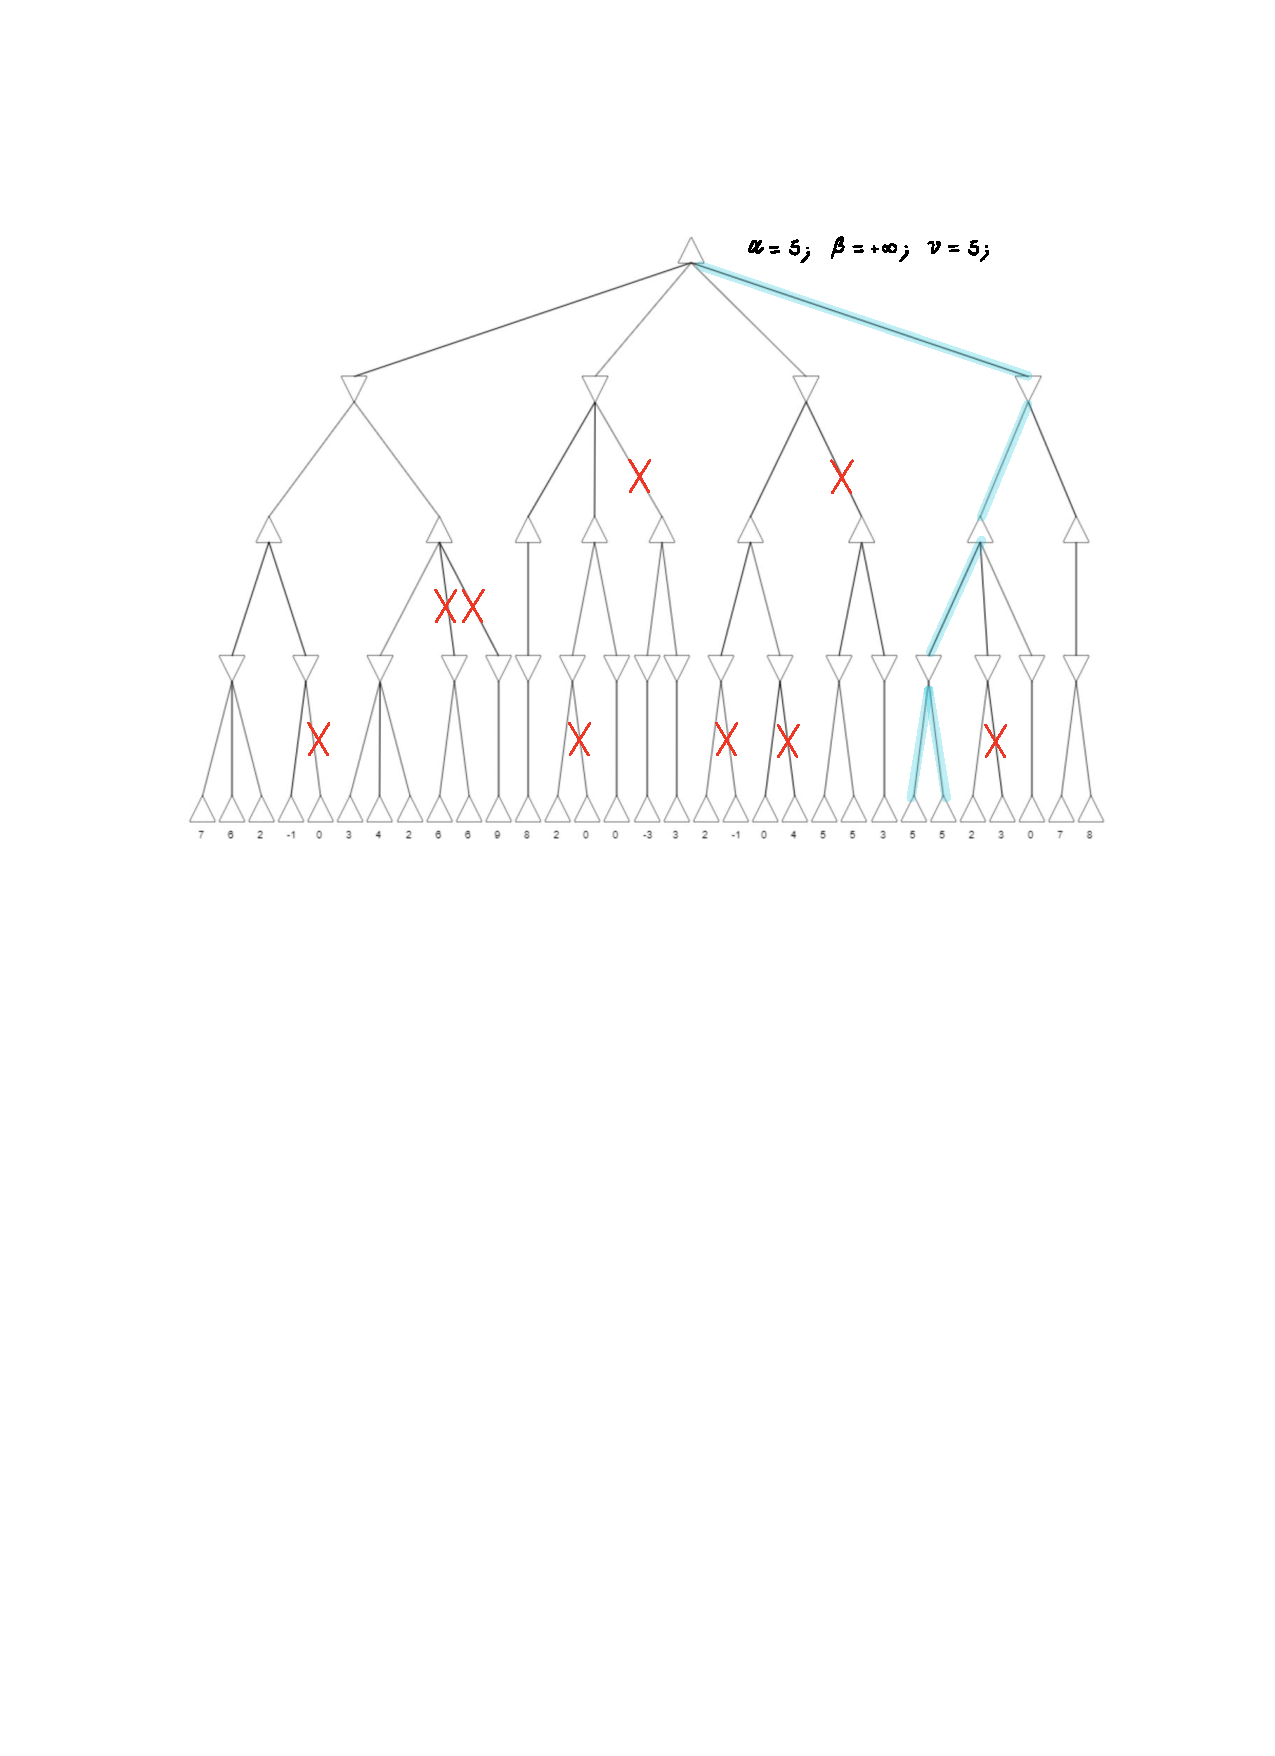
\includegraphics[width=\linewidth]{alpha-beta.pdf}	
		\caption{Alpha-Beta Pruning}
		\label{fig:initial}
	\end{figure}
	
	\newpage
	\section{Genetic Algorithm}
	Write high-level code for a genetic algorithm.
	
	\begin{python}
import numpy as np

# Each gene is a real number between 0 and 1 and corresponds to the 
# probability to have 1 in the corresponding position.
n = 10
P = np.full(n, 0.5)  # initialisation

k = 100
generations = 10
m = 5
condition = True

while condition:
	# Produce a given k number of traditional 0-1 individuals each of 
	# them of length n by sampling gene by gene with the prob vector.
	solution_vector = np.random.binomial(1, P, size=[k, n])
	
	# Evaluate each individual computing the fitness of the 
	# solution_vector
	fitness = evaluate(solution_vector)
	
	# Geerates new individuals
	new_solution_vector = np.empty([k, n])
	
	for i in range(k // 2):
		# Select the best parents in the population for mating
		ind1, ind2 = select_parents(solution_vector, fitness)
		
		# Generate next generation using crossover
		ch1, ch2 = crossover(ind1, ind2)
		
		# Adding some variations to the offsrping using mutation.
		ch1, ch2 = mutate(ch1), mutate(ch2)
		
		new_solution_vector[2*i, :] = ch1
		new_solution_vector[2*i+1, :] = ch2
		
	# At the end of each generation, the best m individuals are used to 
	# update the probabilistic vector.
	fitness = evaluate(new_solution_vector)
	best_individuals = np.argsort(fitness)[::-1][:m]
	
	# For each individual of the best m chosen, the probabilistic vector 
	# is updated using a learning rate LR parameter (real number between 
	# 0 and 1)
	LR = np.random.uniform()
	
	for b in best_individuals:
	P = P * (1.0 - LR) + new_solution_vector[b] * LR
	
	if stop:
	condition = False
\end{python}
	

	
	
	
\end{document}
